\documentclass[12pt,a4paper]{article}
\title{APG4001S Geoid Computation from spherical harmonic coefficients}
\date{10 August 2015}
\author{Tim Marsh}

\usepackage{amsmath}
\usepackage{graphicx}
\usepackage{float}
\usepackage{textcomp}
\usepackage{siunitx}
\usepackage{wrapfig}
\usepackage{caption}
\usepackage{subcaption}



\graphicspath{ {images/} }
\begin{document}
	
	\pagenumbering{gobble}
	\maketitle
	\begin{center}
		\Large Assignment 1
	\end{center}
	
	\begin{figure}[H]
		\centering
		
\includegraphics[width=0.7\linewidth]{UCTcircular_logo1_CMYK}
		\label{fig:UCTcircular_logo1_CMYK}
	\end{figure}
	\newpage
	\pagenumbering{arabic}
	\tableofcontents
	\listoffigures
	
	\newpage
	\section{Introduction}
	
	\subsection{Subject of Report}
	This is a report on Assignment 1 for APG4001S Geodesy. The aim of the report was to calculate orthometric heights for each of the 5 stations provided through the use of spherical harmonic coefficients. 
	
	\subsection{Background}
	Using the GGM02S Grace derived geopotential model, to degree/order 160, and the coordinates of 5 Trignet stations. As well as an exert from the "Geodesists Handbook" which provides the constants required for the GRS80 ellipsoid.
	
	A program is written to calculate the Geoid-ellipsoid (N) values at each station using the geopotential model provided. Using the N value calculate the orthometric height (H) at each station.
	
	\begin{figure}[H]
		\centering
		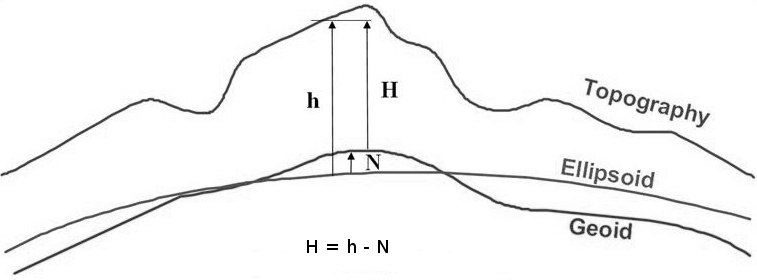
\includegraphics[width=0.7\linewidth]{threeheights_e(1)}
		\caption{Relationship between ellipsoidal height, Geoidal height and orthometric height}
		\label{fig:threeheights}
	\end{figure}
	
	The 5 Trignet stations used are:
	
	\begin{center}
		\begin{tabular}{ | l | l | l | l |}
			\hline
			Station Name & Latitude & Longitude & Ellipsoidal Height \\ \hline
			HNUS & 34 25 28.6671 S & 19 13 23.0264 E &   63.048 \\ \hline
			PRET & 25 43 55.2935 S & 28 16 57.4873 E & 1387.339 \\ \hline
			RBAY & 28 47 43.9616 S & 32 04 42.1896 E &   31.752 \\ \hline
			TDOU & 23 04 47.6714 S & 30 23 02.4297 E &  630.217 \\ \hline
			ULDI & 28 17 35.2196 S & 31 25 15.3309 E &  607.947 \\
			
			\hline
			
		\end{tabular}
	\end{center}
	
	\subsection{Objectives}
	
	The primary objective of this assignment was to create a program to calculate the geoid-ellipsoid values at each station using the provided global geopotential model, once these values are calculated they are used to calculate the orthometric height at each station.	
	
	\subsection{Scope and Limitations}
	
	This assignment was done using the GSM80 ellipsoid and the GGM02S Grace gopotential model to degree/order 160.
	
	A substantial limitation to the program was that Python 3.4 has a size limit on floating point numbers and the code cannot be run for all 160 coefficients without getting an overflow error, so it is only run for 85.
	
	\newpage
	\section{Method}
	
	The program has a reasonably simple structure, the GGM02S file is read in and saved using a class structure in Python 3.4. and is accessible be using a simple query of what you want fed into a function. for example if you want S with n = 57 m = 3 you feed in the query string "S 27 16" and it will return the value 0.39484545087973E-08.
	
	Then for each station a Gamma value for the specific longitude is calculated using the formula:
	
	\begin{equation}
		\gamma = \gamma_e  \frac{n1 + k \sin^2(\Phi)}{\sqrt{1 - e^2 \sin^2(\Phi)}}
	\end{equation}
	\\
	Where $\gamma_e$ is the normal gravity at the equator
	
	\begin{equation}
		N(r, \theta, \lambda) = \frac{GM}{\gamma r} \sum_{n=2}^{\infty} \binom{a}{r} \sum_{m=0}^{n} [(\Delta C_{nm} \cos m\lambda + S_{nm}\sin m\lambda) P_{nm}(\cos\theta)]
	\end{equation}
		
	Them once the $\gamma$ has been calculated, N is calculated in parts. by deconstructing equation (2)  with the inner sum, outer sum and the outermost dividend calculated almost separately and brought together when returned from the function.\\
	\\
	The inner sum which runs inside a loop that runs from 0 to $n$
	\begin{equation}
		InnerSum = \sum_{m=0}^{n} [(\Delta C_{nm} \cos m\lambda + S_{nm}\sin m\lambda) P_{nm}(\cos\theta)]
	\end{equation}
	\\
	In this equation $P_{nm}$ is equal to:
	\begin{equation}
		P_n(t) = \frac{1}{2^n n!} . \frac{d^n}{dt^n} (t^n - 1)^n
	\end{equation}
	Where the value $t = \cos\theta$\\
	\\
	Is then added to the outer sum value and run in a loop from 0 to a specified value, 160.
	
	\begin{equation}
		OuterSum = \sum_{n=2}^{\infty} \binom{a}{r} \times InnerSum
	\end{equation}
	\newpage
	Them finally we add the values that are outside of the outer sum:
	
	\begin{equation}
		N(r, \theta, \lambda) = \frac{GM}{\gamma r} \times OuterSum
	\end{equation}
	\\
	This gives the final value of N.\\
	\\
	Then with this final value of N we calculate the orthometric height with the simple calculation of:
	
	\begin{center}
		Orthometric Height (H) = Ellipsoidal Height (h) - N
	\end{center}
	
	\newpage
	\section{Results}
	The results of calculating N after 85 iterations, n = 85 are as follows: 
	
	\begin{center}
		\begin{tabular}{ | l | c | c |}
			\hline
			Station Name & Orthometric Height & Geoidal Height  \\ \hline
			HNUS &   29.638 & 33.410\\ \hline
			PRET & 1365.770 & 21.569\\ \hline
			TDOU &  611.833 & 18.384\\ \hline
			ULDI &  586.555 & 21.392\\ \hline
			RBAY &   10.520 & 21.232\\
			\hline
			
		\end{tabular}
	\end{center}
	
	These heights are displayed to 3 decimal places, however the program does calculate to around 10 decimal places so the results are rounded of to a usable and more readable size.
	
	As for only doing 85 iterations the later harmonics are making such a small impact of the heights that when rounding off to 3 decimal places no difference will be noticed.
	
	
	
	
	
	
	
	
	
	
	
\end{document}	